Our proposed method for semi-supervised video object segmentation consists of several key steps, which we will outline in detail.
The overall workflow follows a sequential process at each iteration, starting with foreground and background extraction,
followed by ScStream model training, and finally the creation of Gaussian data mixtures to be used in the next iteration.
The central method of our implementation is the \textbf{segment} method in \textcolor{red}{video\_object\_segmentation.py}.
\subsection{First Frame}\label{subsec:first-frame}
\subsubsection{Initial Foreground and Background Extraction}\label{subsubsec:initial-foreground-and-background-extraction}
The first step of our method involves extracting the foreground and background regions from the initial frame of the video.
To accomplish this, we employ the \textbf{GrabCut} algorithm, a popular technique for interactive foreground extraction in images.
The GrabCut algorithm combines color and spatial information to iteratively refine the foreground and background segmentation.
It requires an initial bounding box or a rough mask specifying the location of the foreground object.
In our case, this a great option to define the ground-truth mask of the object in the first video frame, since it is a semi-supervised method.
Our implementation of GrabCut uses the OpenCV library and can be found in the \textcolor{red}{grab\_cut.py} file.
Example result:
\begin{figure}[h!]
    \begin{minipage}{0.5\textwidth}
    \centering
    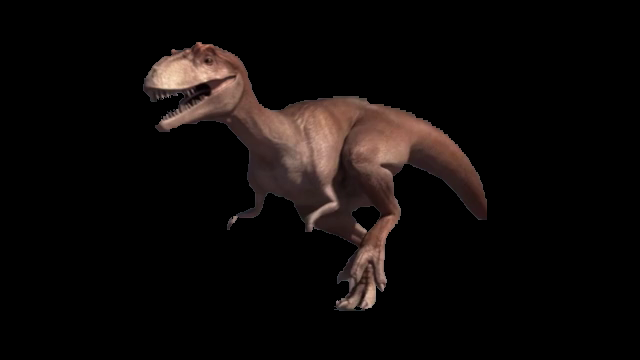
\includegraphics[scale=0.4]{images/dinosaur/foreground_ratio1.0}
    \caption{Foreground}
    \end{minipage}
    \begin{minipage}{0.5\textwidth}
    \centering
    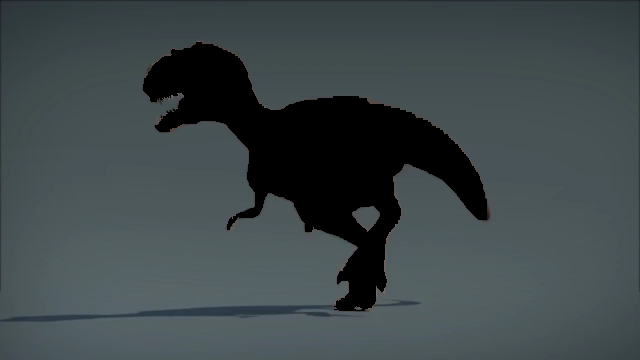
\includegraphics[scale=0.4]{images/dinosaur/background_ratio1.0}
    \caption{Background}
    \end{minipage}\label{fig:foreground extraction}
\end{figure}

\subsubsection{Models Initialization}
Once the foreground and background regions of the current frame have been extracted, we proceed to initialize our models.
Our goal is to be able to classify data to foreground and background by their characteristics.
Therefore, creating a model for each of them will create two separate and different gaussians that we can later extract from the models and use as our classifiers.
When initializing our models with \texttt{fit\_init} we have to do some hyper-parameter tuning that we will discuss in the next section.
Also, we want to let \texttt{fit\_init} run until convergence, since the initial run is on the ground-truth data and we want the model to learn it accurately.
\pagebreak
\subsection{Segmentation Loop}\label{subsec: segment-loop}
\subsubsection{Creation of Gaussian Data Mixtures}\label{subsubsec:gaussians}
As previously said the gaussians of the foreground and background models are our classifiers, helping us determine how to separate a new frame into 2 parts.
we can build them by extracting the means and covariances of the clusters from each model and initialize a \textbf{GaussianMixture} instance for both of them.
The GaussianMixture class is defined in \textcolor{red}{gaussian\_mixture.py} and uses \texttt{Scipy.stats.multivariate\_normal} to represent each gaussian.
The class supports two pdf options, pdf of the mixture using weights and sum of all gaussians pdfs, and max pdf that returns the gaussian pdf with the largest value.
\lstinputlisting[language=Python, firstline=7, lastline=20,label={lst:gaussians}]{../gaussian_mixture.py}
\subsubsection{Foreground and Background Extraction}\label{subsubsec: fg-bg-extract}
Now that we can no longer supervise the separation of the foreground and background we need to define a decision rule
that exploits the given gaussianMixtures and classifies each pixel in the new frame into foreground and background.
This is the most time-consuming part of our loop as we need to go over every pixel and calculate its pdfs.
Further discussion about the decision rule will be in the next section.

\subsubsection{Model adjustment}\label{subsubsec:model-adjust}
Given we have a new foreground and background we should utilize them to update our models, given it is very likely that our object changed its position from the previous frame.
The updated models will provide new gaussian mixtures that should classify the next frame better than the previous mixtures.
The adjustment stage will also be discussed in the next section.
\pagebreak

\subsection{Building The Segmented Video}\label{subsec:build-segment-video}
At each iteration we produce foreground and background images for each frame, which we can use to build a segmented video.
To highlight the foreground object, we can apply a color mask to the foreground image.
The color mask is simply a binary mask with the same dimensions as the foreground image, where the foreground pixels are set to green and the background pixels are set to black.
Then using the OpenCV library, we can apply the color mask to the original frame to highlight the foreground object.
This is implemented in the \textbf{classify\_frame} method in \textcolor{red}{video\_object\_segmentation.py}.
\begin{figure}[h!]
    \centering
    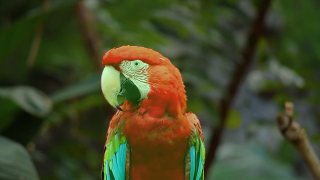
\includegraphics[scale=1.5]{new_frames/dinosaur_best/frame0}
    \caption{Segmented first frame}
    \label{fig:segmented-video}
\end{figure}

